%%%%%%%%%%%%%%%%%%%%%%%%%%%%%%%%%%%%%%%%%
% Beamer Presentation
% LaTeX Template
% Version 1.0 (10/11/12)
%
% This template has been downloaded from:
% http://www.LaTeXTemplates.com
%
% License:
% CC BY-NC-SA 3.0 (http://creativecommons.org/licenses/by-nc-sa/3.0/)
%
%%%%%%%%%%%%%%%%%%%%%%%%%%%%%%%%%%%%%%%%%

%----------------------------------------------------------------------------------------
%	PACKAGES AND THEMES
%----------------------------------------------------------------------------------------

\documentclass{beamer}

\mode<presentation> {
	
	% The Beamer class comes with a number of default slide themes
	% which change the colors and layouts of slides. Below this is a list
	% of all the themes, uncomment each in turn to see what they look like.
	
	%\usetheme{default}
	%\usetheme{AnnArbor}
	%\usetheme{Antibes}
	%\usetheme{Bergen}
	%\usetheme{Berkeley}
	%\usetheme{Berlin}
	%\usetheme{Boadilla}
	%\usetheme{CambridgeUS}
	%\usetheme{Copenhagen}
	%\usetheme{Darmstadt}
	%\usetheme{Dresden}
	%\usetheme{Frankfurt}
	%\usetheme{Goettingen}
	%\usetheme{Hannover}
	%\usetheme{Ilmenau}
	%\usetheme{JuanLesPins}
	%\usetheme{Luebeck}
	\usetheme{Madrid}
	%\usetheme{Malmoe}
	%\usetheme{Marburg}
	%\usetheme{Montpellier}
	%\usetheme{PaloAlto}
	%\usetheme{Pittsburgh}
	%\usetheme{Rochester}
	%\usetheme{Singapore}
	%\usetheme{Szeged}
	%\usetheme{Warsaw}
	
	% As well as themes, the Beamer class has a number of color themes
	% for any slide theme. Uncomment each of these in turn to see how it
	% changes the colors of your current slide theme.
	
	%\usecolortheme{albatross}
	\usecolortheme{beaver}
	%\usecolortheme{beetle}
	%\usecolortheme{crane}
	%\usecolortheme{dolphin}
	%\usecolortheme{dove}
	%\usecolortheme{fly}
	%\usecolortheme{lily}
	%\usecolortheme{orchid}
	%\usecolortheme{rose}
	%\usecolortheme{seagull}
	%\usecolortheme{seahorse}
	%\usecolortheme{whale}
	%\usecolortheme{wolverine}
	
	%\setbeamertemplate{footline} % To remove the footer line in all slides uncomment this line
	%\setbeamertemplate{footline}[page number] % To replace the footer line in all slides with a simple slide count uncomment this line
	
	%\setbeamertemplate{navigation symbols}{} % To remove the navigation symbols from the bottom of all slides uncomment this line
}

\usepackage{graphicx} % Allows including images
\usepackage{subfigure}
\usepackage{booktabs} % Allows the use of \toprule, \midrule and \bottomrule in tables
\usepackage{bm}

%----------------------------------------------------------------------------------------
%	TITLE PAGE
%----------------------------------------------------------------------------------------

\title[ASPCA]{On Consistency and Sparsity for PCA in High Dimensions} 

\author{Ganchao Wei} 
\date{October 20, 2021}

\begin{document}
	
	\begin{frame}
		\titlepage % Print the title page as the first slide
	\end{frame}
	
	\begin{frame}
		\frametitle{Overview} % Table of contents slide, comment this block out to remove it
		\tableofcontents
	\end{frame}
	
	%--------------------------------------------------------------------
	%	PRESENTATION SLIDES
	%--------------------------------------------------------------------
	
	\section{Introduction}
	
	\begin{frame}
		\frametitle{Introduction}
		In regular PCA, we assume $n \gg p$. However, in many situations, $p$ is comparable in magnitude with $n$ or even $n < p$ (high-dimensional settings). In this paper, they:
		\begin{itemize}
			\item
			describe inconsistency results to emphasize that when $p$ is comparable with $n$, we need to reduce dimension.
			\item
			establish consistency results to illustrate that the reduction in dimensionality ca be effected working in a basis in which the signals have a sparse representation.
		\end{itemize}
		\textbf{Setting}: single factor model
		$$\bm{x}_i=\nu_i\bm{\rho} + \sigma\bm{z}_i,\,\, i=1,\ldots,n$$
		, where $\bm{x}_i \in \mathbb{R}^p$,  $\bm{\rho} \in \mathbb{R}^p$, $\nu_i\sim N(0,1)$ and $\bm{z}_i\sim N_p(0,I)$
	\end{frame}
	
	\begin{frame}
		\frametitle{Introduction: Motivating Example}
		$$\bm{x}_i=\nu_i\bm{\rho} + \sigma\bm{z}_i,\,\, i=1,\ldots,n$$
		,where $p=2048, n= 1024$. The vector $\rho_l=f(l/p)$ for $l\in {1,\ldots,p}$, and $f(t)$ is a mixture of beta desnities on $[0,1]$, scaled so that $||\bm{\rho}||_2 = 10$. Specifically, $f(t) = C{0.7Beta(1500,3000) + 0.5Beta(1200,900) + 0.5Beta(600,160)}$. The $\sigma=1$. Here, they analyzed the data by 4 different methods (results in the next slide):
		\begin{itemize}
			\item
			standard PCA
			\item
			smoothed PCA: similar to LASSO, add penalty terms, i.e. maximize
			$$var(\bm{\xi}'\bm{x}_i)/[||\bm{\xi}||^2 + \lambda ||D^2\bm{\xi}||^2]$$
			\item
			adaptive sparse PCA, without thresholding (this paper)
			\item
			adaptive sparse PCA, with thresholding (this paper)
		\end{itemize} 
	\end{frame}
	
	\begin{frame}
		\frametitle{Introduction: Motivating Example}
		\begin{figure}
			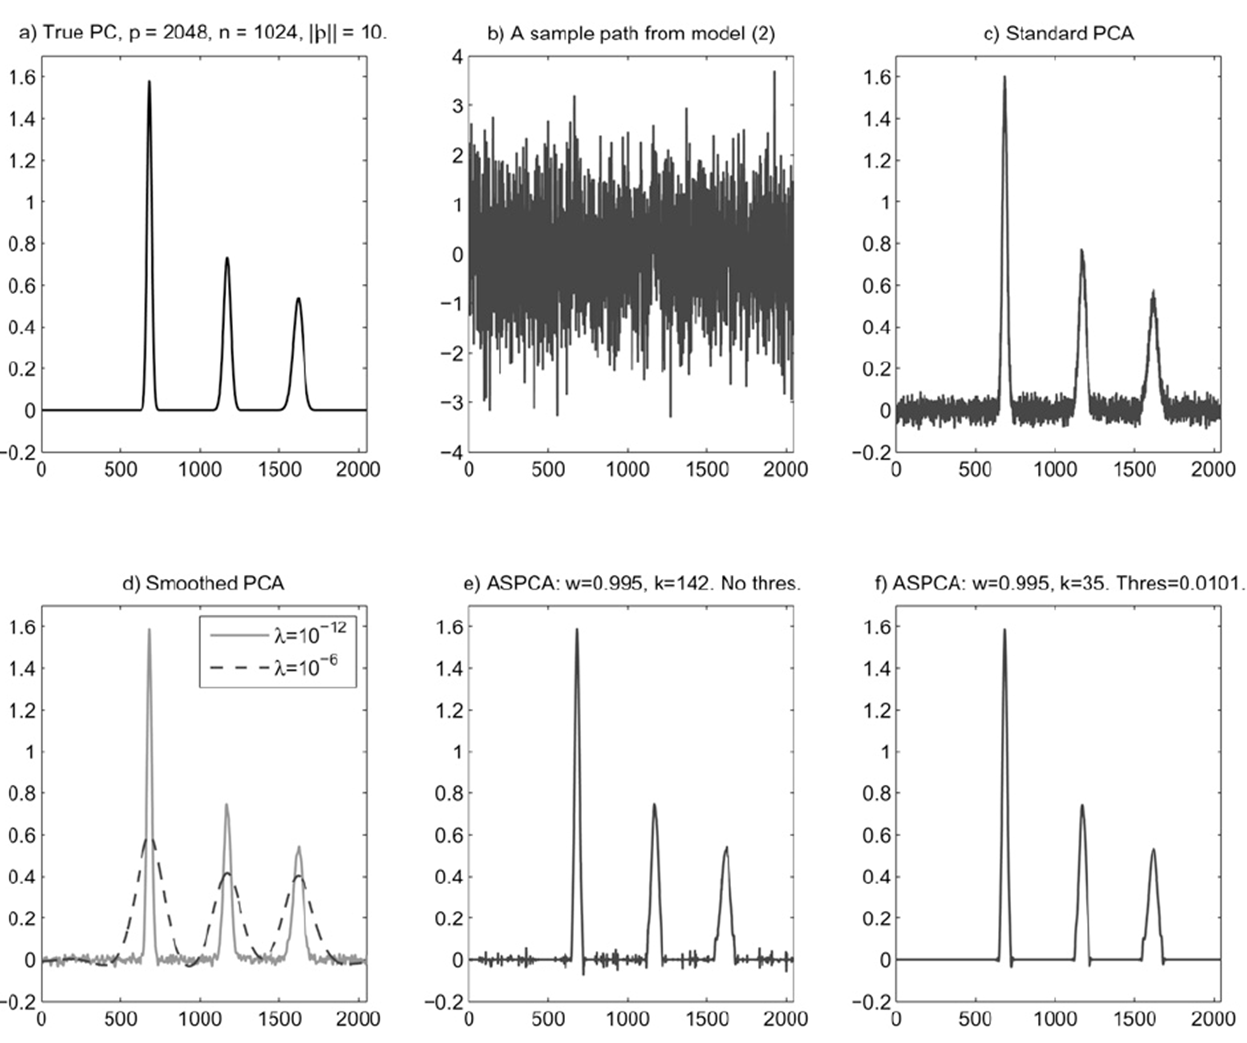
\includegraphics[width=0.8\linewidth]{image001.png}
		\end{figure}
	\end{frame}
	
	\section{Inconsistency}
	\begin{frame}
		\frametitle{Inconsistency of Classic PCA}
		First, some notations \& definitions:
		\begin{itemize}
			\item
			$\bm{S}$ = sample covariance, $\hat{\bm{\rho}}$ = eigenvectors with largest eigenvalue
			\item
			overlap between 2 vectors: $R(\hat{\bm{\rho}}, \bm{\rho}) = \cos \angle(\hat{\bm{\rho}}, \bm{\rho})$
			\item
			distance: $d(\hat{\bm{\rho}}, \bm{\rho}) = \sin \angle(\hat{\bm{\rho}}, \bm{\rho})$
		\end{itemize}
		We also need 2 more assumptions:
		\begin{itemize}
			\item
			dimension growth: $\lim_{n \to \infty}p_n/n = c$
			\item
			limiting SNR: $\lim_{n \to \infty} ||\bm{\rho}_n||^2/\sigma^2 = \omega>0$
		\end{itemize}
	\end{frame}
	
	
	\begin{frame}
		\frametitle{Inconsistency of Classic PCA}
		This leads to the limiting results (Theorem 1)
		\begin{figure}
			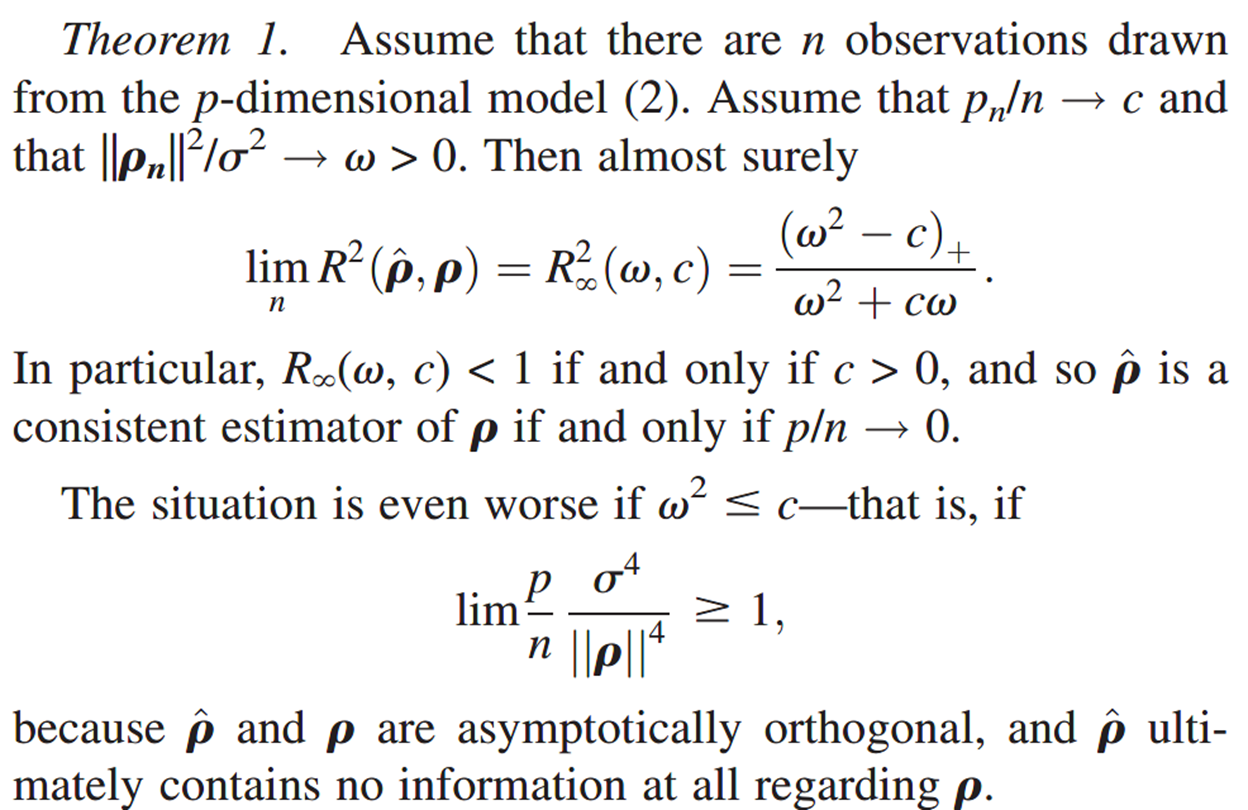
\includegraphics[width=0.8\linewidth]{image002.png}
		\end{figure}
		The theorem can be easily extended to the multi-component case.
	\end{frame}
	
	\section{Sparsity, Selection and Consistency}
	\begin{frame}
		\frametitle{Sparsity}
		Theorem 1 tells us that regular PCA becomes confused when there are too many variables each with equal independent noise $\Rightarrow$ reduce dimension.\\
		Assume the data and population PC's are represented in a fixed orthonormal basis  ${\bm{e}_{\nu}}$ (maybe after transformation):
		\begin{figure}
			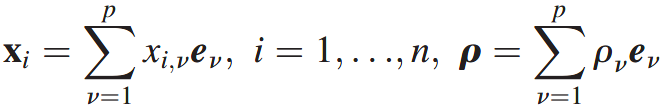
\includegraphics[width=0.5\linewidth]{image003.png}
		\end{figure}
		Denote the ordered magnitutes as $|\rho|_{(1)} \geq |\rho|_{(2)} \geq \ldots$ We further need the magnitudes decay rather quickly:
		$$|\rho|_{(\nu)} \leq C\nu^{-1/q}$$
		,where $0<q<2$ and $C>0$.
		
		In other words, we want the "energy" in the largest $k$ coordinates $\sum_{i=1}^{k}\rho^2_{(i)}$ is close to the total energy $||\bm{\rho}||^2$.
	\end{frame}
	
	
	\begin{frame}
		\frametitle{Consistency}
		To show consistency after selection, we assume: (1) each of unknown $\bm{\rho} = \bm{\rho}_n$ decays fast; (2) stable signal strength: $||\bm{\rho}_n|| \to \varrho > 0$.
		The sample variances:
		\begin{figure}
			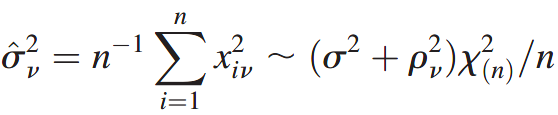
\includegraphics[width=0.5\linewidth]{image004.png}
		\end{figure}  
		So, larger values of $\rho_v$ will typically have larger sample variances. This leads to a simple selection rule:
		$$\hat{I} = \{{\nu: \hat\sigma}^2_{\nu} \geq \sigma^2(1+\alpha_n)\}$$
		, with $\alpha_n = \alpha(n^{-1}\log(n \vee p))^{1/2}$.
	\end{frame}
	
	
	\begin{frame}
		\frametitle{Consistency}
		Let $\bm{S}_I = (S_{\nu\nu'}: \nu\, \text{and}\, \nu' \in \hat{I})$ denote the sample covariance of the selected variables. Then apply regular PCA to $\bm{S}_I$. Let $\hat{\bm{\rho}}_I$ denote the corresponding vector in the full p-dimensional space:
		\begin{figure}
			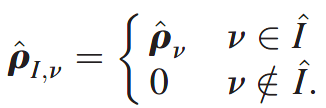
\includegraphics[width=0.3\linewidth]{image005.png}
		\end{figure}
	\end{frame}
	
	\begin{frame}
		\frametitle{Consistency}
		Under this selection, they show consistency after selection (Theorem 2):
		\begin{figure}
			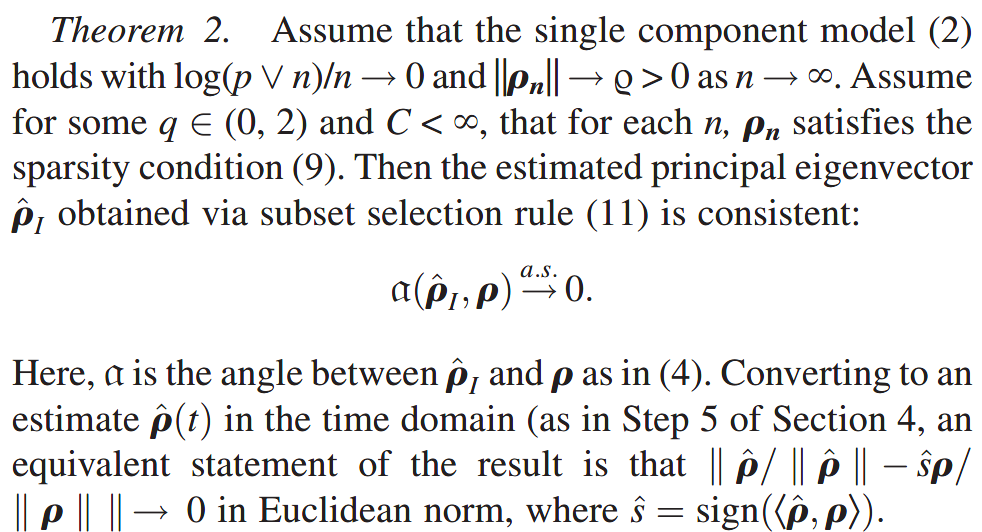
\includegraphics[width=0.8\linewidth]{image006.png}
		\end{figure}
	\end{frame}
	
	\begin{frame}
		\frametitle{Correct Selection Properties}
		\textbf{Question}: Do the selected subset $\hat{I}$ in fact correctly contains the largest \textbf{population} variances? And only those (no false inclusion)?\\
		For this section, assume sample (coordinate) variance have marginal $\chi^2$ distribution:
		$$\hat{\sigma}^2_{\nu} = S_{\nu\nu}\sim \sigma^2_{\nu}\chi^2_{(n)}/n$$
		Denote the orderd population \& sample coordinate variance as $\sigma^2_{(1)}\geq \sigma^2_{(2)}\geq\ldots$ and $\hat{\sigma}^2_{(1)}\geq \hat{\sigma}^2_{(2)}\geq\ldots$. And further denote:
		\begin{itemize}
			\item
			$I_{in} = \{l:\sigma^2_l \geq \sigma^2_{(k)}(1+\alpha_n)\}$
			\item
			$I_{out} = \{l:\sigma^2_l \leq \sigma^2_{(k)}(1+\alpha_n)\}$
			\item
			false exclusion (FE): $FE = \cup_{l\in I_{in}} \{\hat{\sigma}^2_l < \hat{\sigma}^2_{(k)}\}$
			\item 
			false inclusion (FI): $FI = \cup_{l\in I_{out}} \{\hat{\sigma}^2_l \geq \hat{\sigma}^2_{(k)}\}$
		\end{itemize}
	\end{frame}
	
	\begin{frame}
		\frametitle{Correct Selection Properties}
		The correct selection properties are shown in Theorem 3:
		\begin{figure}
			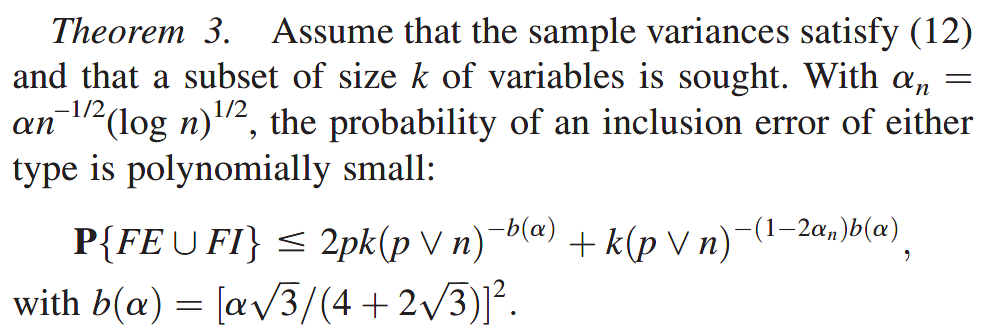
\includegraphics[width=0.8\linewidth]{image007.png}
		\end{figure}
		
	\end{frame}
	
	\section{Illustrative Algorithm}
	\begin{frame}
		\frametitle{An Illustrative Algorithm}
		\begin{figure}
			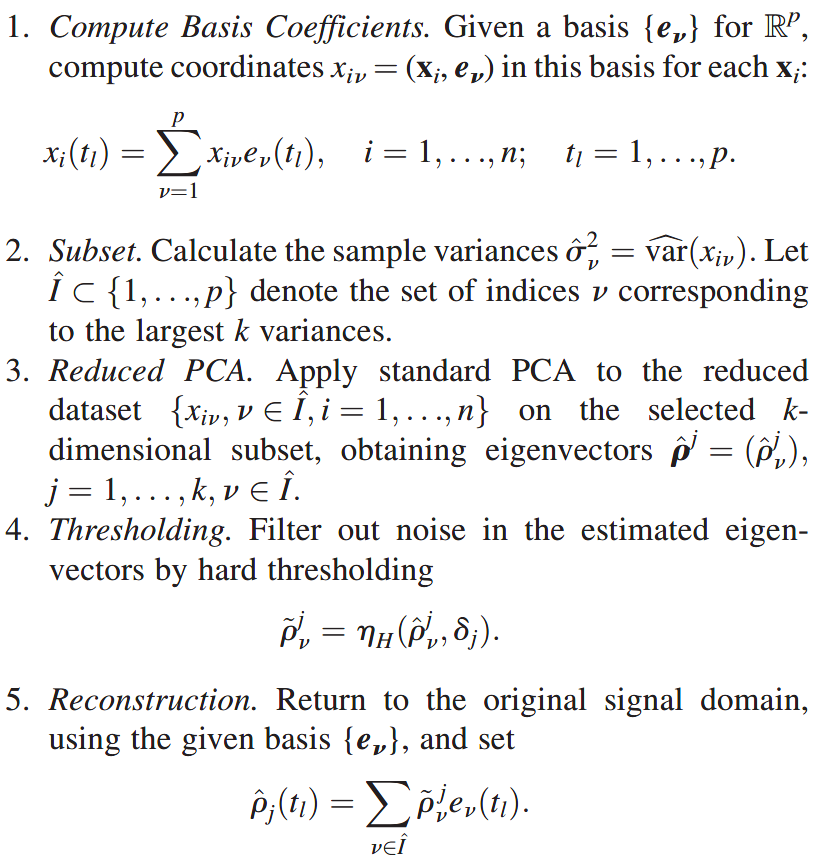
\includegraphics[width=0.6\linewidth]{image008.png}
		\end{figure}
	\end{frame}
	
	\begin{frame}
		\frametitle{An Illustrative Algorithm}
		Some comments about thresholding:
		\begin{itemize}
			\item
			hard thresholding: $\eta_H(y,\delta) = yI\{|y| \geq \delta\}$
			\item 
			choose $\delta_j$: by analogy with the signal in Gaussian noies setting $\delta_j = \hat{\tau}_j\sqrt{2\log k}$
			\item
			$\hat{\tau}_j$ is an estimate of the noise level in $\{\hat{\rho}^j_{\nu}, \nu\in\hat{I}\}$
			\item
			In this paper, they estimate it as $\hat{\tau}\approx \frac{1}{\sqrt{n}}\frac{\sigma\sqrt{||\bm{\rho}||^2 + \sigma^2}}{||\bm{\rho}||^2}$. This is derived from the asymptotic distribution of $\hat{\bm{\rho}}$. $||\bm{\rho}||^2$ and $\sigma^2$ can be estimated by data.
			\item
			We can also do things as $\hat{\tau}_j = MAD\{\hat{\rho}^j_{\nu}, \nu\in\hat{I}\}/0.6745$
		\end{itemize}
	\end{frame}
	
	
	\begin{frame}
		\frametitle{Data-based Choice of $k$ and estimation of $\sigma$}
		The paper provides 2 possibilities:
		\begin{itemize}
			\item
			shown in previous:  $\hat{I} = \{{\nu: \hat\sigma}^2_{\nu} \geq \sigma^2(1+\alpha_n)\}$
			\item
			Define
			\begin{figure}
				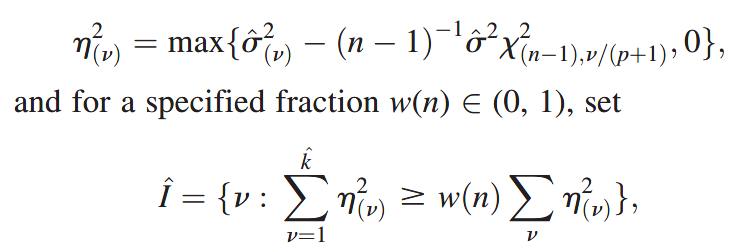
\includegraphics[width=0.7\linewidth]{image009.png}
			\end{figure}
		\end{itemize}
		\textbf{Estimation of $\sigma$}:\\
		If the population PC have a sparse representation, then in most coordinates, $\nu$, $x_{i\nu}$ will consist largely of noise.
		Then we can estimate $\sigma$ as:
		$$\hat{\sigma}^2 = median(\hat{\sigma}^2_{\nu})$$
	\end{frame}
	
	\section{Examples}
	\begin{frame}
		\frametitle{Simulations}
		The first simulation ("3-peak") is shown in the motivation example. Here, they further show another ("step") example.
		\begin{figure}
			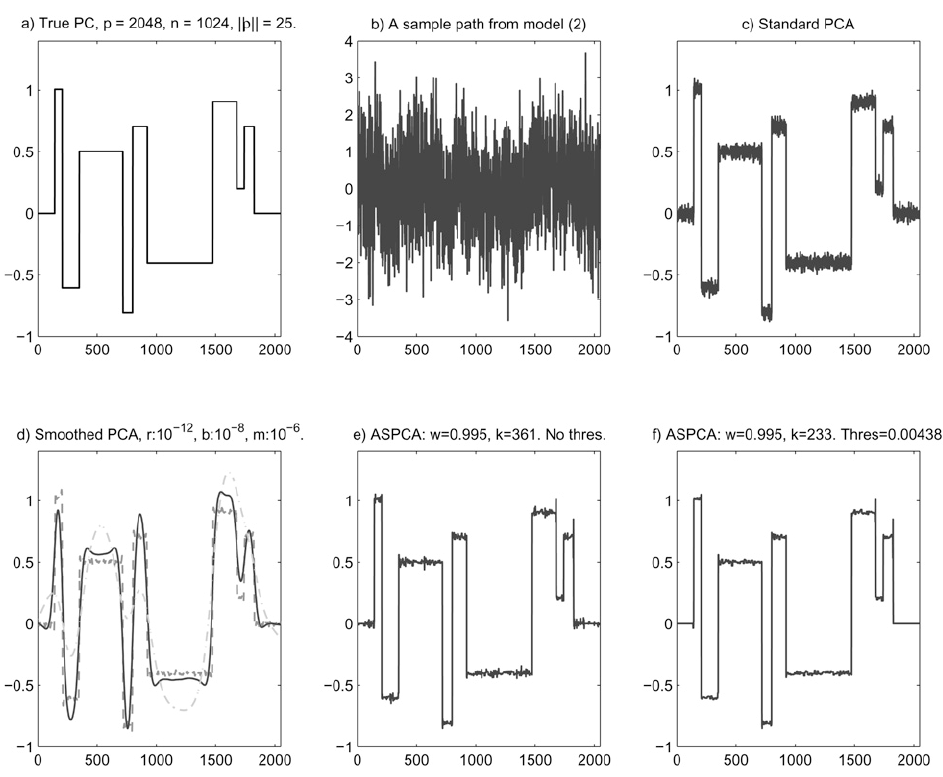
\includegraphics[width=0.7\linewidth]{image010.png}
		\end{figure}
		
	\end{frame}


	\begin{frame}
		\frametitle{Simulations}
	The average squared error (ASE) is defined as $ASE = p^{-1}||\hat{\bm{\rho}} - \bm{\rho}||$. The comparisons among different methods:
	\begin{figure}
		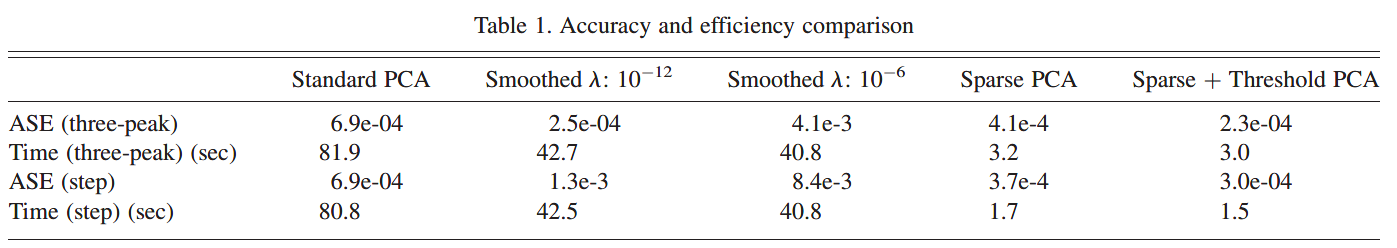
\includegraphics[width=0.9\linewidth]{image011.png}
		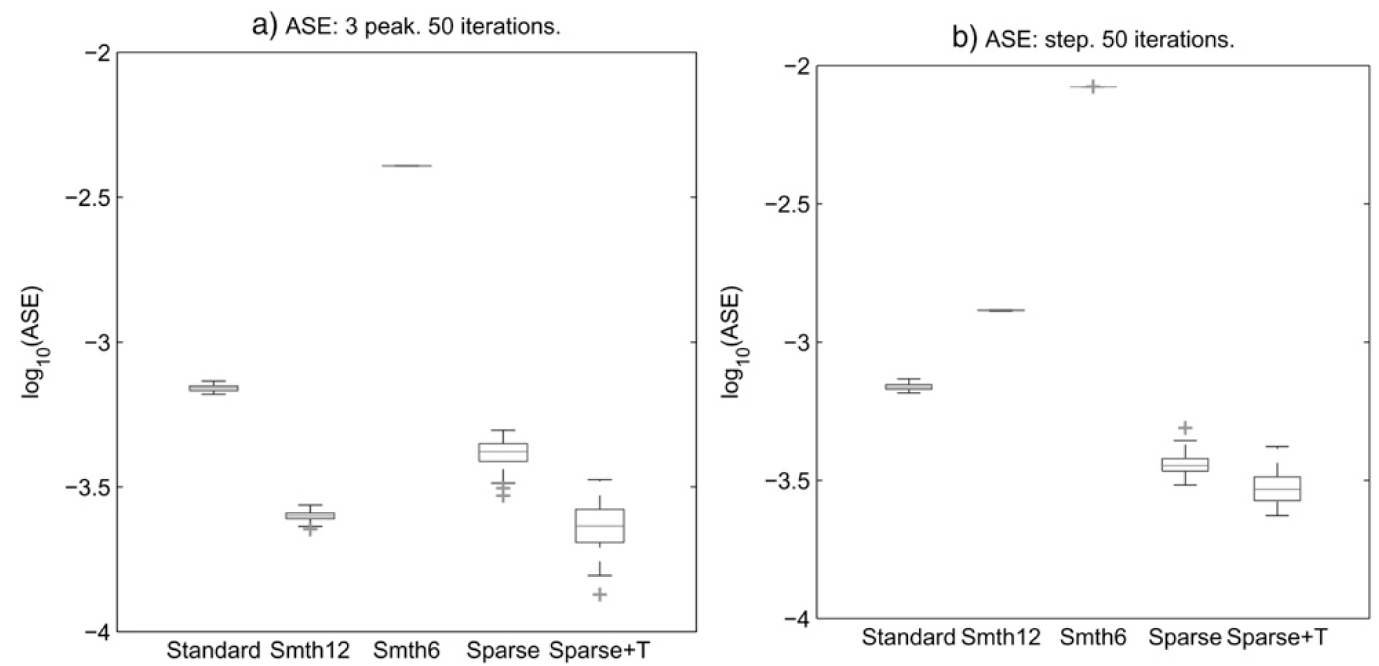
\includegraphics[width=0.8\linewidth]{image012.png}
	\end{figure}
	\end{frame}

	\begin{frame}
		\frametitle{ECG Example}
		\begin{figure}
			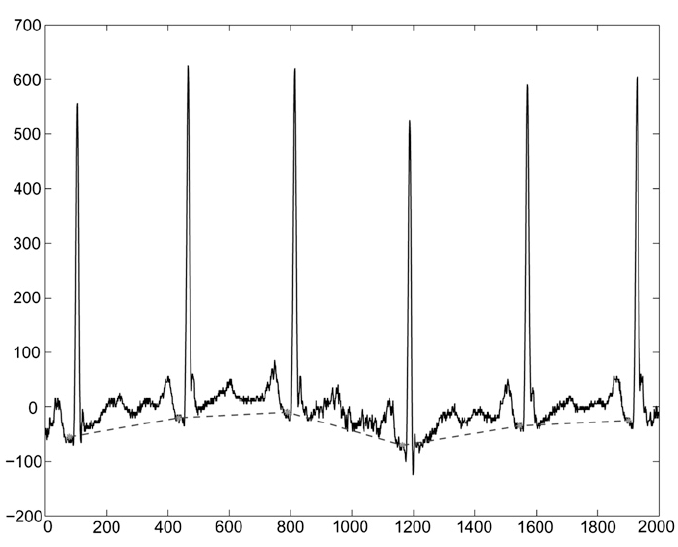
\includegraphics[width=0.5\linewidth]{image013.png}
		\end{figure}
		\begin{itemize}
			\item 
			The ECG data has "baseline wander", and this is adjusted by piece-wise linear baseline.
			\item
			Each individual betas are combined by sharp spike ("QRS complex", max at R wave) + lower peak ("T wave")
		\end{itemize}
		
	\end{frame}



	\begin{frame}
		\frametitle{ECG Example}
		After prepossessing (e.g. adjust baseline wander and align peaks),  they converted the ECG data vector to a $n \times 512$ matrix. $n$ is the number of cycle, $p=512$ is the duration of the cycle. The wavelet base is used here.
		\begin{figure}
			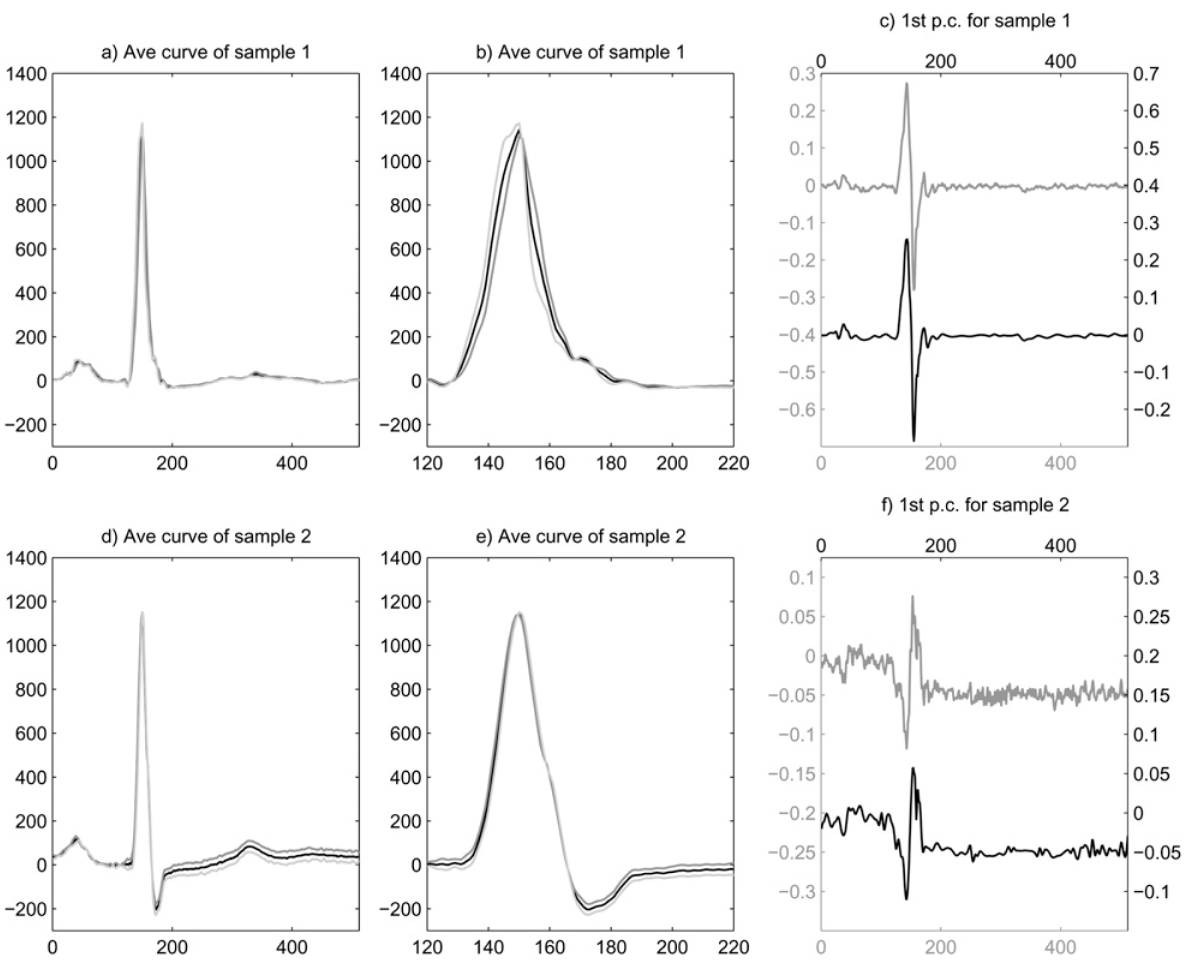
\includegraphics[width=0.6\linewidth]{image014.png}
		\end{figure}
		The SPCA is less noisy while keeping the features.
	\end{frame}

	
	
	
	
	
	
	
\end{document}